\documentclass{beamer}

\usepackage[british]{babel}
\usepackage{graphicx,hyperref,ru,url,xcolor}


% The title of the presentation:
%  - first a short version which is visible at the bottom of each slide;
%  - second the full title shown on the title slide;
\title[Lock-in Feedback for Sequential Experiments]{
  Lock-in Feedback for Sequential Experiments}

% Optional: a subtitle to be dispalyed on the title slide
\subtitle{by Maurits Kaptein \& Davide Iannuzzi}

% The author(s) of the presentation:
%  - again first a short version to be displayed at the bottom;
%  - next the full list of authors, which may include contact information;
\author[Schmidl \& Kemper]{
  Christoph Schmidl - s4226887 \\ Chris Kemper - s4359410\\}

% The institute:
%  - to start the name of the university as displayed on the top of each slide
%    this can be adjusted such that you can also create a Dutch version
%  - next the institute information as displayed on the title slide
\institute[Radboud University Nijmegen]{
  Master AI \\
  Radboud University Nijmegen}

% Add a date and possibly the name of the event to the slides
%  - again first a short version to be shown at the bottom of each slide
%  - second the full date and event name for the title slide
\date[29 November 2017]{
  29 November 2017}

\begin{document}

\begin{frame}
  \titlepage
\end{frame}



% Section titles are shown in at the top of the slides with the current section 
% highlighted. Note that the number of sections determines the size of the top 
% bar, and hence the university name and logo. If you do not add any sections 
% they will not be visible.
\section{Introduction}

\begin{frame}
  \frametitle{General Opinion}
  \begin{itemize}
    \item Well structured
    \item Easy to understand
    \item Clear real world applications
    \item Inadequate comparisons
  \end{itemize}
\end{frame}

\section{Summary}

\begin{frame}
  \frametitle{Lock-in Feedback}
  
   
    \begin{figure}
            \centering
            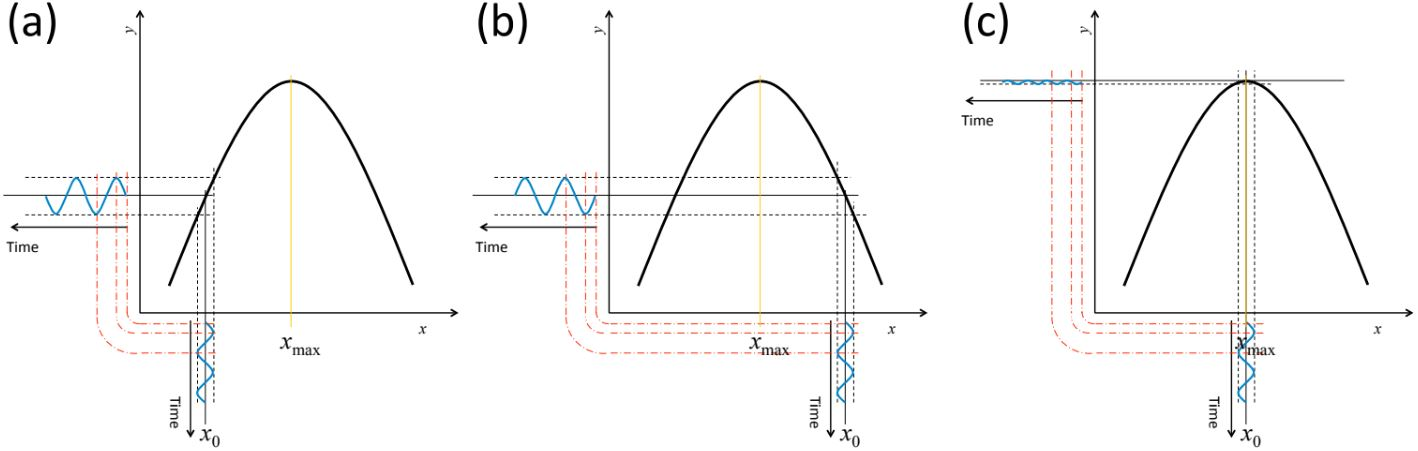
\includegraphics[width=\textwidth]{images/General_Idea}
            \label{fig:alg}
        \end{figure}

  \begin{block}{The basis}
    \begin{itemize}
      \item Find maximum of unknown function
      \item Inspired by Lock-in amplifiers
    \end{itemize}
  \end{block}
\end{frame}

\begin{frame}
    \frametitle{Algorithm}
    
    \begin{figure}
            \centering
            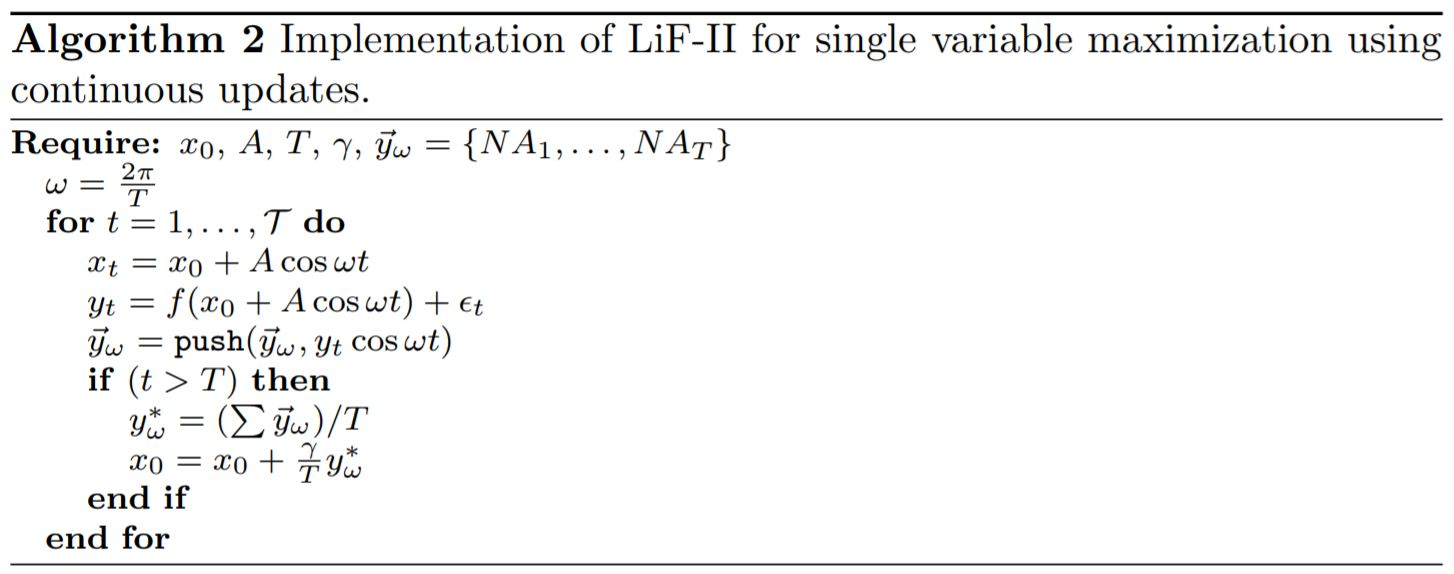
\includegraphics[width=\textwidth]{images/algorithm}
            \label{fig:alg}
        \end{figure}
\end{frame}

\begin{frame}
    \frametitle{Simulation 2 - Noise}
     
    \begin{figure}
            \centering
            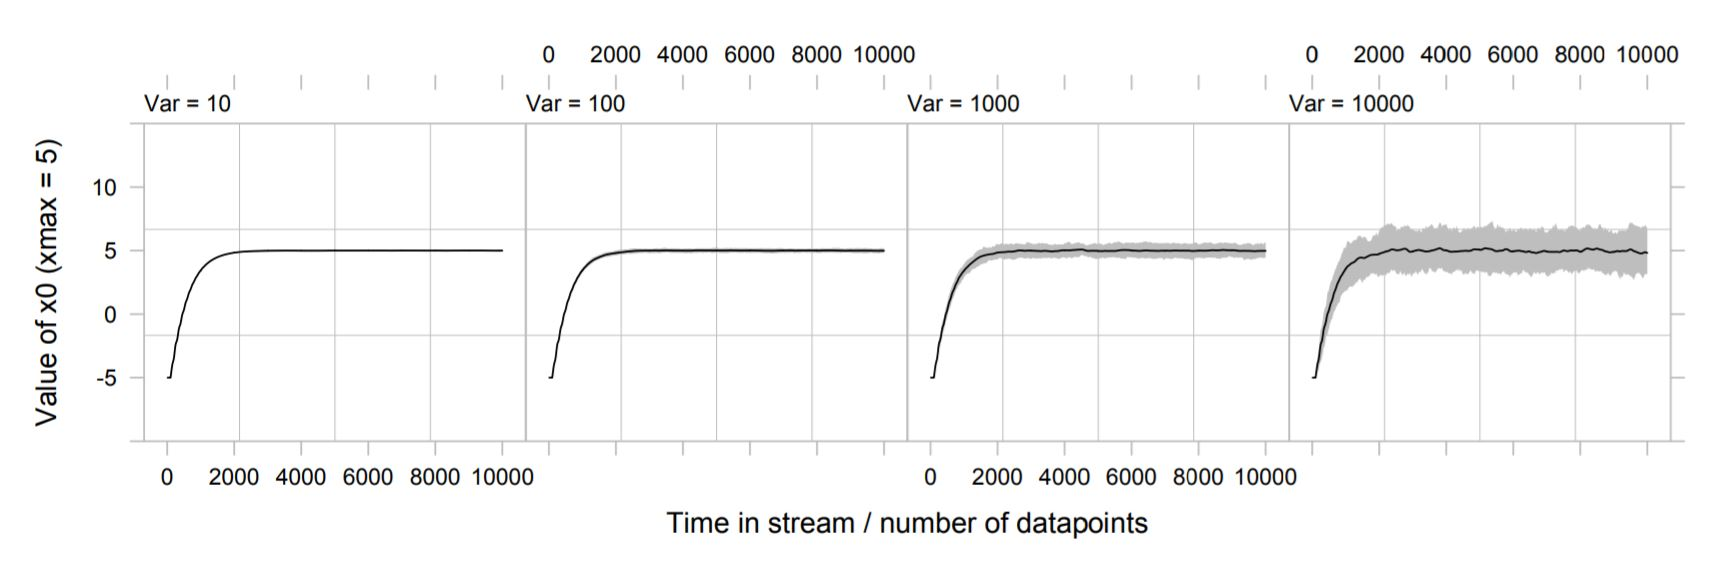
\includegraphics[width=\textwidth]{images/sim_2}
            \label{fig:alg}
        \end{figure}
\end{frame}

\begin{frame}
    \frametitle{Simulation 3 - Concept Drift} 
    \begin{figure}
            \centering
            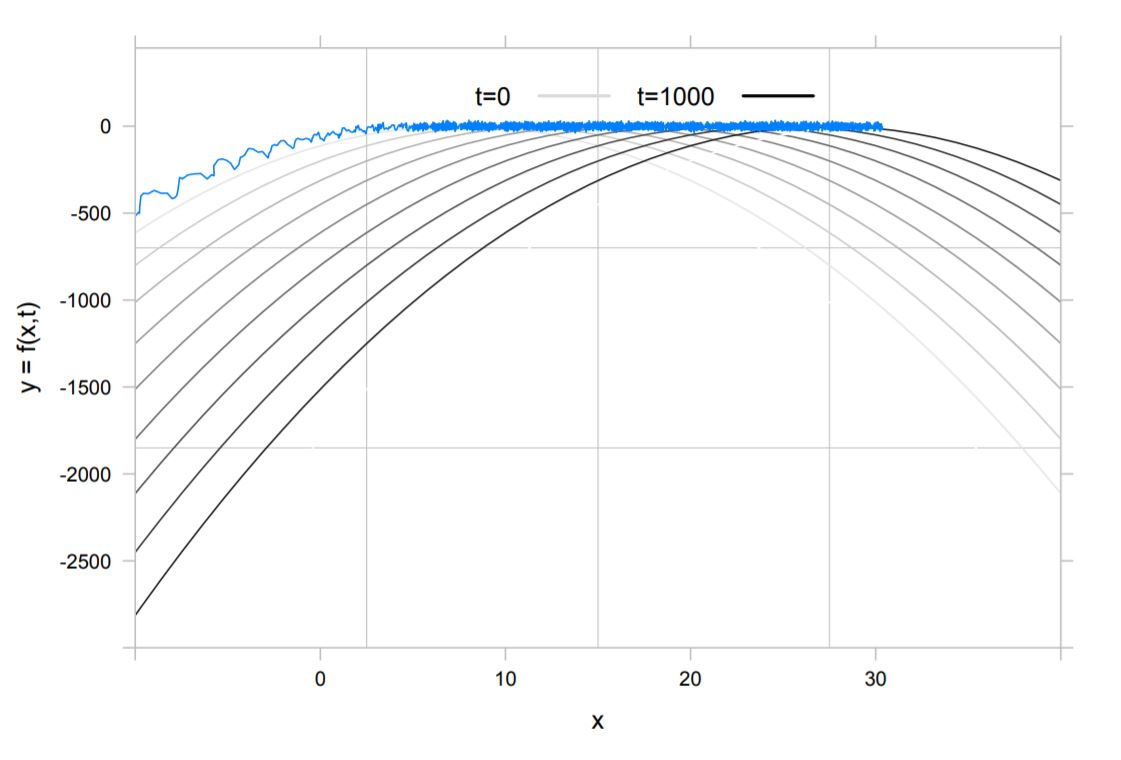
\includegraphics[width=\textwidth]{images/sim_3}
            \label{fig:alg}
        \end{figure}
\end{frame}

\begin{frame}
    \frametitle{Simulation 4 - Dichotomous observations}
     
    \begin{figure}
            \centering
            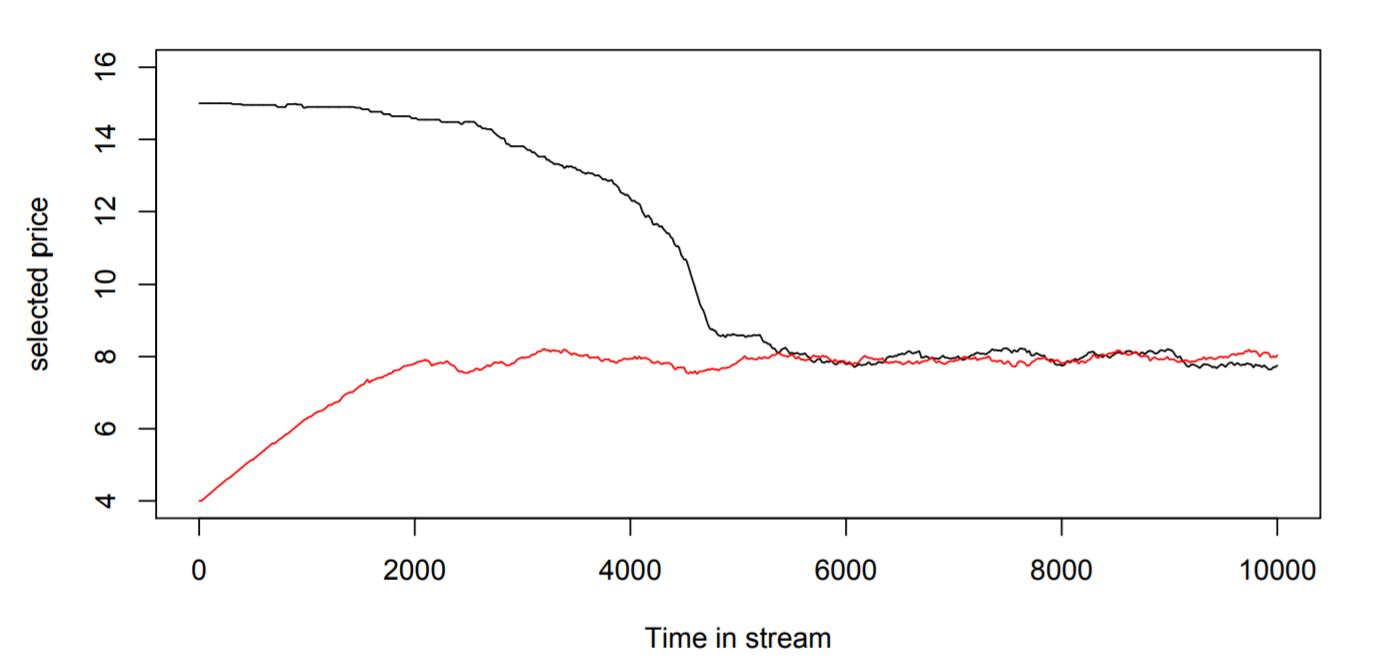
\includegraphics[width=\textwidth]{images/sim_4}
            \label{fig:alg}
        \end{figure}
\end{frame}

\begin{frame}
    \frametitle{Simulation 5 - Comparison}
     
    \begin{figure}
            \centering
            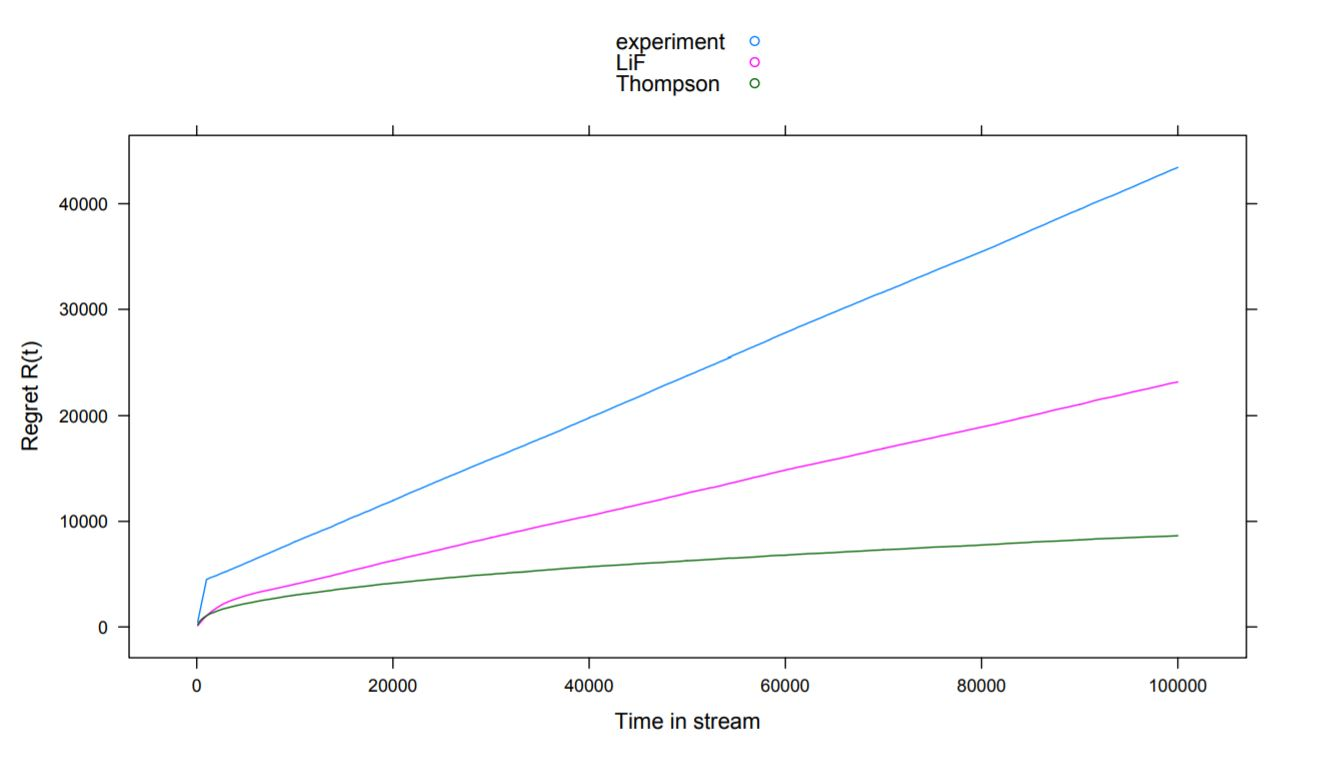
\includegraphics[width=\textwidth]{images/sim_5}
            \label{fig:alg}
        \end{figure}
\end{frame}

\begin{frame}
    \frametitle{Conclusion}
    \begin{itemize}
        \item Derivative free method to find maxima
        \item Deals well with noise and concept drift
        \item Can be expanded to multivariate problems
    \end{itemize}
\end{frame}

\section{Reflection}

\begin{frame}
  \frametitle{Critique}
    \begin{block}{Pros}
      \begin{itemize}
        \item Well structured
        \item Easy to understand
        \item Clear real world applications
      \end{itemize}
    \end{block}
  \begin{block}{Cons}
    \begin{itemize}
      \item Inadequate comparisons
    \end{itemize}
  \end{block}
\end{frame}

\begin{frame}
    \frametitle{Comparison}
     
    \begin{figure}
            \centering
            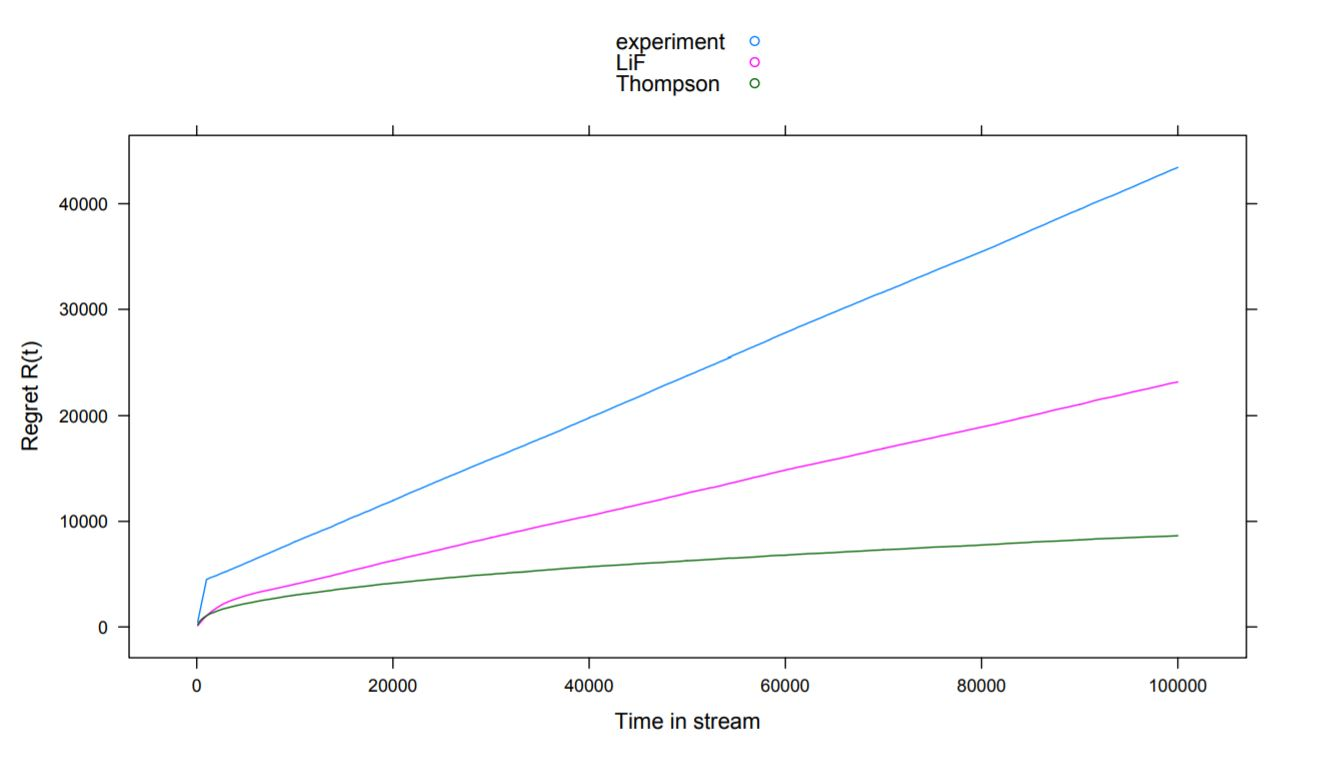
\includegraphics[width=\textwidth]{images/sim_5}
            \label{fig:alg}
        \end{figure}
\end{frame}

\begin{frame}
    \frametitle{Comparison}
     \begin{figure}
            \centering
            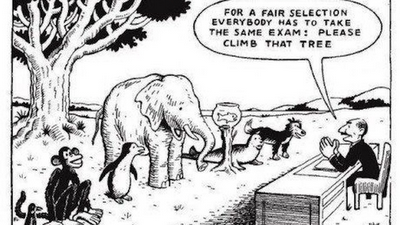
\includegraphics[width=\textwidth]{images/fishtree.png}
            \label{fig:alg}
        \end{figure}
\end{frame}


\begin{frame}
    \frametitle{Further work}
    \begin{block}{Adaptive approach to concept drift}
        \begin{itemize}
            \item Decrease amplitude to 0 at intervals
            \item Increase size of intervals if no concept drift is found
        \end{itemize}
    \end{block}
    \begin{block}{Multivariate functions}
    \begin{itemize}
        \item Complexity doesn't increase with variables
        \item Multiple variables most likely increase noise
    \end{itemize}
    \end{block}
\end{frame}

\section{Conclusion}

\begin{frame}
  \frametitle{Conclusion}
  \begin{itemize}
      \item Well structured
      \item Easy to understand
      \item Might be useful in real world scenarios 
  \end{itemize}
  \begin{center}
  \textcolor{red}{\textbf{Don't measure the intelligence of a fish by its ability to climb a tree}}
  \end{center}

\end{frame}


\begin{frame}{Discussion 1: Local Maxima}
    \begin{itemize}
        \item Multiple methods possible: random walks, momentum, multiple starting points
        \item All methods increase regret in first steps
    \end{itemize}
    
\end{frame}

\begin{frame}{Discussion 2: Applications in Medicine}
    \begin{itemize}
        \item Takes regret into account from the start
        \item Performs very well on small number of patients
        \item Difficult to incorporate some physiological traits
    \end{itemize}
    
\end{frame}

\begin{frame}{Discussion 3: Extending to Multivariate Problems}
    \begin{itemize}
        \item Oscillate all variables at different frequencies
        \item Make inferences about the lone variables
    \end{itemize}
\end{frame}

\begin{frame}
    \frametitle{Discussion 3: Extending to Multivariate Problems}
    
    \begin{figure}
            \centering
            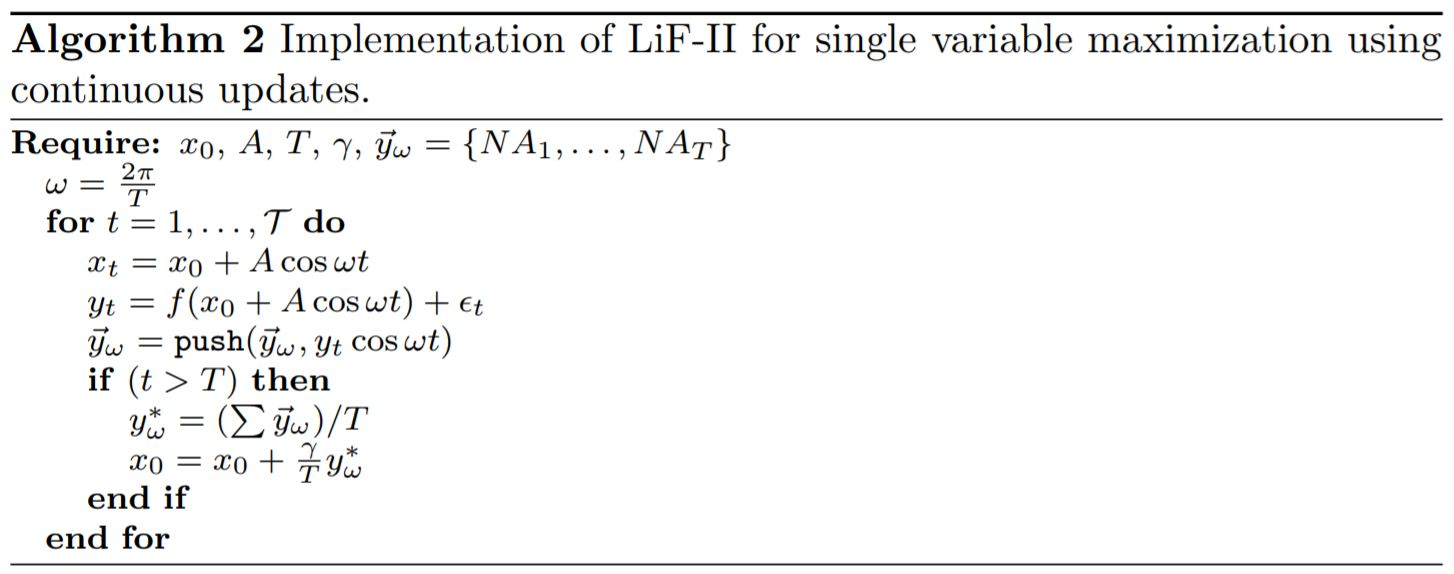
\includegraphics[width=\textwidth]{images/algorithm}
            \label{fig:alg}
        \end{figure}
\end{frame}

\begin{frame}{Momentum}
    \begin{figure}
            \centering
            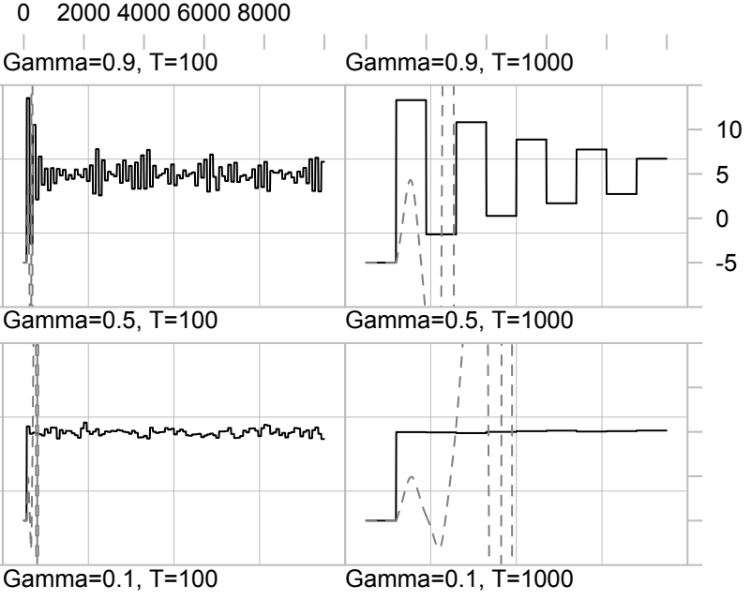
\includegraphics[width=0.7\textwidth]{images/momentum}
            \label{fig:alg}
        \end{figure}
\end{frame}

\end{document}
